\documentclass[letterpaper]{memoir}
\usepackage{tikz}
\usepackage{geometry}
\geometry{letterpaper,left=0pt,top=0pt,right=0pt,bottom=0pt}
\usetikzlibrary{calc}

\begin{document}
	% Material Design Palette, Purple 700
	\definecolor{front}{RGB}{123,31,162}
	% Material Design Palette, Purple 600
	\definecolor{left}{RGB}{142,36,170}
	% Material Design Palette, Purple 400
	\definecolor{top}{RGB}{171,71,188}
	
	\begin{center}
		\begin{vplace}
			\begin{tikzpicture}[y={(-0.5cm,0.25cm)},x={(0.5cm,0.25cm)},z={(0cm,0.5cm)}]
			% C
			\draw[fill=front] (0,0,0) -- (3,0,0) -- (3,0,1) -- (1,0,1) -- (1,0,4) -- (3,0,4) -- (3,0,5) -- (0,0,5) -- (0,0,0);
			\draw[fill=left] (0,0,0) -- (0,1,0) -- (0,1,5) -- (0,0,5) -- cycle;
			\draw[fill=top] (0,0,5) -- (0,1,5) -- (3,1,5) -- (3,0,5) -- cycle;
			\draw[fill=top] (3,0,1) -- (3,1,1) -- (2,1,1) -- (1,0,1) -- cycle;
			% A
			\draw[fill=front] (4,0,0) -- (4,0,5) -- (7,0,5) -- (7,0,0) -- (6,0,0) -- (6,0,2) -- (5,0,2) -- (5,0,0) -- cycle;
			\draw[fill=white] (5,0,3) -- (5,0,4) -- (6,0,4) -- (6,0,3) -- cycle;
			\draw[fill=left] (4,0,0) -- (4,1,0) -- (4,1,5) -- (4,0,5) -- cycle;
			\draw[fill=top] (4,0,5) -- (4,1,5) -- (7,1,5) -- (7,0,5) -- cycle;
			\draw[fill=left] (6,0,3) -- (6,1,3) -- (6,0,4) -- cycle;
			\draw[fill=top] (5,0,3) -- (6,0,3) -- (6,1,3) -- cycle;
			\draw[fill=left] (6,0,0) -- (6,1,0) -- (6,1,1) -- (6,0,2) -- cycle;
			% L
			\draw[fill=front] (8,0,0) -- (8,0,5) -- (9,0,5) -- (9,0,1) -- (11,0,1) -- (11,0,0) -- cycle;
			\draw[fill=left] (8,0,0) -- (8,1,0) -- (8,1,5) -- (8,0,5) -- cycle;
			\draw[fill=top] (8,1,5) -- (8,0,5) -- (9,0,5) -- (9,1,5) -- cycle;
			\draw[fill=top] (11,0,1) -- (11,1,1) -- (10,1,1) -- (9,0,1) -- cycle;
			% E
			\draw[fill=front] (12,0,0) -- (12,0,5) -- (15,0,5) -- (15,0,4) -- (13,0,4) -- (13,0,3) -- (15,0,3) -- (15,0,2) -- (13,0,2) -- (13,0,1) -- (15,0,1) -- (15,0,0) -- cycle;
			\draw[fill=left] (12,0,0) -- (12,1,0) -- (12,1,5) -- (12,0,5) -- cycle;
			\draw[fill=top] (12,0,5) -- (12,1,5) -- (15,1,5) -- (15,0,5) -- cycle;
			\draw[fill=top] (15,0,3) -- (15,1,3) -- (14,1,3) -- (13,0,3) -- cycle;
			\draw[fill=top] (15,0,1) -- (15,1,1) -- (14,1,1) -- (13,0,1) -- cycle;
			% N
			\draw[fill=front] (16,0,0) -- (16,0,5) -- (17,0,5) -- (18,0,2.5) -- (18,0,5) -- (19,0,5) -- (19,0,0) -- (18,0,0) -- (17,0,2.5) -- (17,0,0) -- cycle;
			\draw[fill=left] (16,0,0) -- (16,1,0) -- (16,1,5) -- (16,0,5) -- cycle;
			\draw[fill=top] (16,0,5) -- (16,1,5) -- (17,1,5) -- (17,0,5) -- cycle;
			\draw[fill=top] (18,0,5) -- (18,1,5) -- (19,1,5) -- (19,0,5) -- cycle;
			\draw[fill=left] (18,1,5) -- (17,0,5) -- (18,0,2.5) -- (18,0,5) -- cycle;
			\draw[fill=left] (18,0,0) -- (18,1,0) -- (17,0,2.5) -- cycle;
			% D
			\draw[fill=front] (20,0,0) -- (20,0,5) -- (22,0,5) -- (23,0,4) -- (23,0,1) -- (22,0,0) -- cycle;
			\draw[fill=white] (21,0,1) -- (21,0,4) -- (22,0,4) -- (22,0,1) -- cycle;
			\draw[fill=left] (20,0,0) -- (20,1,0) -- (20,1,5) -- (20,0,5) -- cycle;
			\draw[fill=top] (20,0,5) -- (20,1,5) -- (22,1,5) -- (22,0,5) -- cycle;
			\draw[fill=left] (22,0,1) -- (22,1,1) -- (21,0,4) -- (22,0,4) -- cycle;
			\draw[fill=top] (21,0,1) -- (22,1,1) -- (22,0,1) -- cycle;
			% A
			\draw[fill=front] (24,0,0) -- (24,0,5) -- (27,0,5) -- (27,0,0) -- (26,0,0) -- (26,0,2) -- (25,0,2) -- (25,0,0) -- cycle;
			\draw[fill=white] (25,0,3) -- (25,0,4) -- (26,0,4) -- (26,0,3) -- cycle;
			\draw[fill=left] (24,0,0) -- (24,1,0) -- (24,1,5) -- (24,0,5) -- cycle;
			\draw[fill=top] (24,0,5) -- (24,1,5) -- (27,1,5) -- (27,0,5) -- cycle;
			\draw[fill=left] (26,0,3) -- (26,1,3) -- (26,0,4) -- cycle;
			\draw[fill=top] (25,0,3) -- (26,0,3) -- (26,1,3) -- cycle;
			\draw[fill=left] (26,0,0) -- (26,1,0) -- (26,1,1) -- (26,0,2) -- cycle;
			% R
			\draw[fill=front] (28,0,0) -- (28,0,5) -- (31,0,5) -- (31,0,2) -- (30.5,0,2) -- (31,0,0) -- (30,0,0) -- (29.5,0,2) -- (29,0,2) -- (29,0,0) -- cycle;
			\draw[fill=left] (28,0,0) -- (28,1,0) -- (28,1,5) -- (28,0,5) -- cycle;
			\draw[fill=top] (28,0,5) -- (28,1,5) -- (31,1,5) -- (31,0,5) -- cycle;
			\draw[fill=left] (30,0,3) -- (30,1,3) -- (30,0,4) -- cycle;
			\draw[fill=top] (29,0,3) -- (29,0,4) -- (30,0,3) -- cycle;
			\draw[fill=left] (30,0,0) -- (30,1,0) -- (29,0,2) -- (29.5,0,2) -- cycle;
			\end{tikzpicture}
	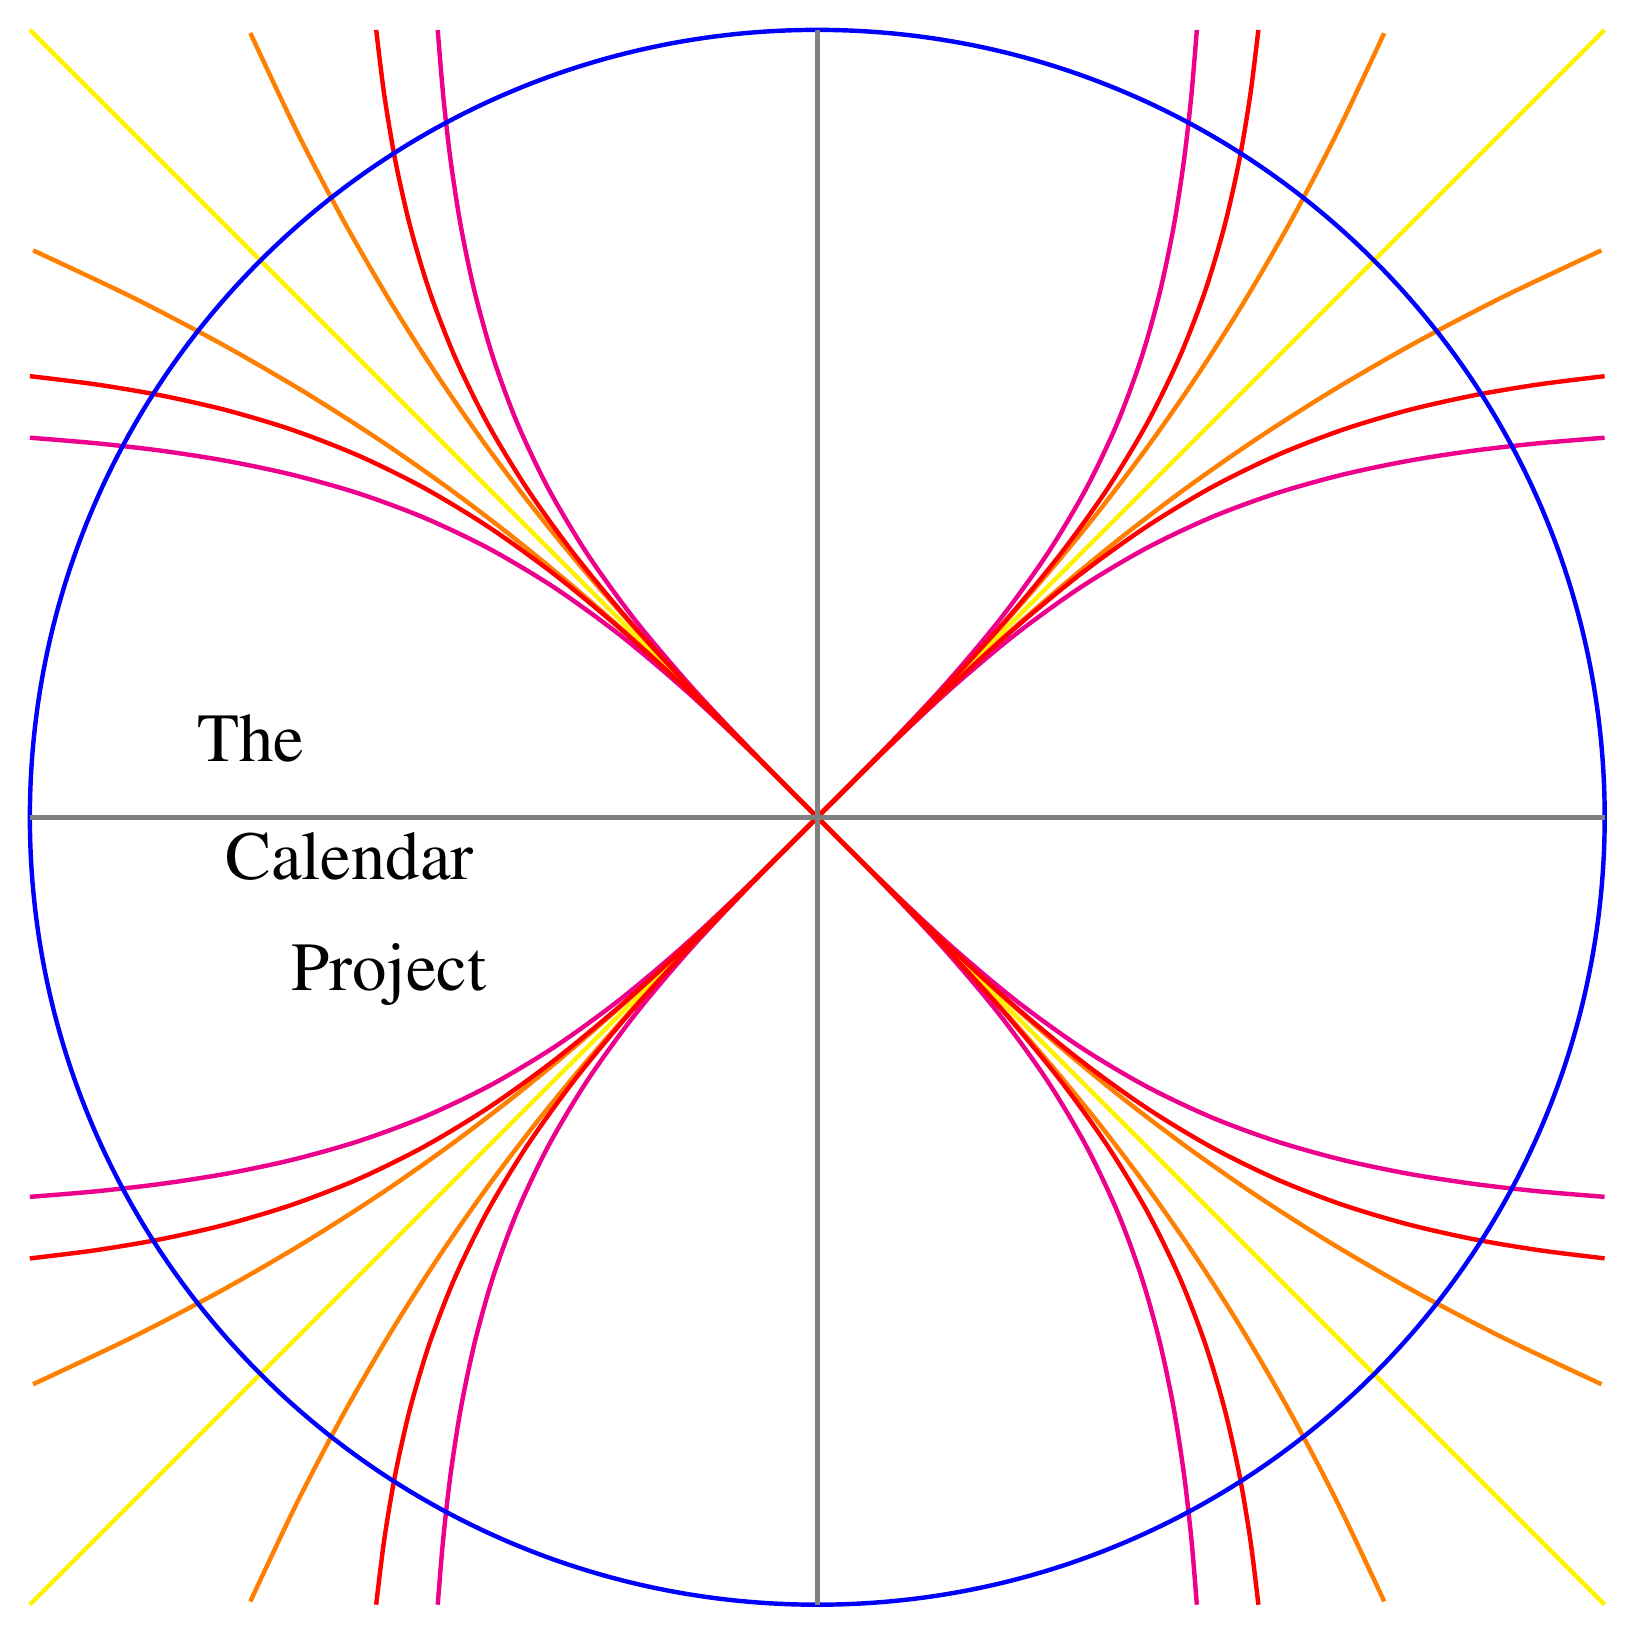
\begin{tikzpicture}[xscale=5,yscale=5]
		\draw[domain=-2:2,smooth,ultra thick,magenta] plot ({\x},{tanh \x});
		\draw[domain=-2:2,smooth,ultra thick,yellow] plot ({\x}, {\x});
		\draw[domain=-2:2,smooth,ultra thick,yellow] plot ({\x}, {-\x});
		\draw[domain=-2:2,smooth,ultra thick,magenta] plot ({\x},{-tanh \x});
		\draw[domain=-2:2,smooth,ultra thick,variable=\y,magenta] plot ({tanh \y},{\y});
		\draw[domain=-2:2,smooth,ultra thick,variable=\y,magenta] plot ({-tanh \y},{\y});
		\draw[domain=-1.44:1.44,smooth,ultra thick,orange] plot ({\x},{sinh \x});
		\draw[domain=-1.44:1.44,smooth,ultra thick,variable=\y,orange] plot ({sinh \y},{\y});
		\draw[domain=-1.44:1.44,smooth,ultra thick,orange] plot ({\x},{-sinh \x});
		\draw[domain=-1.44:1.44,smooth,ultra thick,variable=\y,orange] plot ({-sinh \y},{\y});
		\draw[domain=-2:2,smooth,ultra thick,red] plot ({\x},{sinh (tanh \x)});
		\draw[domain=-2:2,smooth,ultra thick,variable=\y,red] plot ({sinh (tanh \y)},{\y});
		\draw[domain=-2:2,smooth,ultra thick,red] plot ({\x},{-sinh (tanh \x)});
		\draw[domain=-2:2,smooth,ultra thick,variable=\y,red] plot ({-sinh (tanh \y)},{\y});
		\draw[ultra thick,blue] (0,0) circle [radius=2];
		\draw[ultra thick,gray] (-2,0) -- (2,0);
		\draw[ultra thick, gray] (0,2) -- (0,-2);
		\node at (-1.45,0.2) {\fontfamily{ptm} \Huge The};
		\node at (-1.2,-0.1) {\fontfamily{ptm} \Huge Calendar};
		\node at (-1.1,-0.4) {\fontfamily{ptm} \Huge Project};
	\end{tikzpicture}
	\end{vplace}
	\end{center}
\end{document}